\documentclass[11pt, twocolumn]{article}

\usepackage[margin=1in]{geometry}
\usepackage{booktabs}
\usepackage{multirow}
\usepackage{tabularx}
\usepackage{pgf}
\usepackage{amsmath,amssymb}
\usepackage[utf8]{inputenc}
\usepackage[page]{appendix}
\usepackage{textcase}
\usepackage{setspace}
\usepackage{scalefnt}
\usepackage{url}
\usepackage{graphicx}
\usepackage{hyperref}
%\usepackage{fancyhdr}

\setcounter{secnumdepth}{1}
\renewcommand{\baselinestretch}{1.1}

\setlength{\parindent}{0pt} 
\setlength{\parskip}{1.5ex}

%%%%%%%%%%%%%%%%%%%%%%%%%
% Title Page Info
%%%%%%%%%%%%%%%%%%%%%%%%%

\title{ENSC 483 - Project 2: Magnetic Levitation Control}

%\prof{Professor Mahdi Alavi}

\date{April 28, 2010}

\begin{document}
\begin{titlepage}
	\vspace*{2em}
	\begin{center}
		{\Huge ENSC 483 - Project 2: Magnetic Levitation Control}
	\end{center}
	\null\vfill

	\vskip 2em

	\begin{center}
		{\Large
		Dan Hendry (danh@sfu.ca), 301133878\\
   		Veronica Cojocaru (vca5@sfu.ca), 301055896
   		}
	\end{center}
	\vskip 2em
	
	\begin{center}
		{Simon Fraser University \\
		School of Engineering Science}
	\end{center}
	\vskip 2em

	\begin{center}
		{April 28, 2010\\
		Course Instructor: Professor Mahdi Alavi}
	\end{center}
\end{titlepage}

\cleardoublepage

\pagenumbering{arabic}

%%%%%%%%%%%%%%%%%%%%%%%%%
% Main Section
%%%%%%%%%%%%%%%%%%%%%%%%%

%Add chapters as needed

\section{Introduction}

What are we doing.

Attractive levitation.

Design state feedback and observer.

Not using the observer for control: why - stupid machine.

\subsection{System Model}

Matricies and values

\subsection{Initial pole locations and stability}

Current location of the poles

\section{State Feedback}

The first step was to stabilize the system using state feedback

\subsection{System Model}

Formulation of state feedback

\subsection{Desired pole location}

For overshoot and settling time

\subsection{Gain Determination}

Getting k from desired pole location

\section{Observer}

An observer was then designed

\subsection{System Model}

TODO

\subsection{Gain Determination}

TODO

\chapter{Results}

\section{Success Rate}

\subsection{Simulation 1}

\begin{figure}[h!]
    \centering
    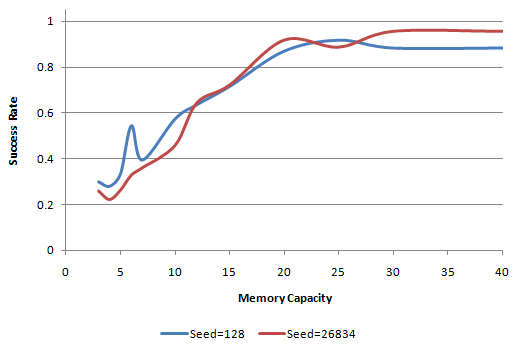
\includegraphics[width=.9\textwidth]{images/result_sccess_sim1byseed_dss}
    \caption{TODO}
    %\label{fig:moistureSensor}
\end{figure}

\subsection{Simulation 2}

\begin{figure}[h!]
    \centering
    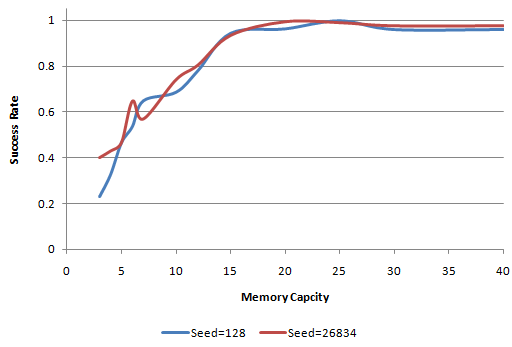
\includegraphics[width=.9\textwidth]{images/result_sccess_sim2byseed_dss}
    \caption{TODO}
    %\label{fig:moistureSensor}
\end{figure}

\subsection{Comparison of Success Rate}

\begin{figure}[h!]
    \centering
    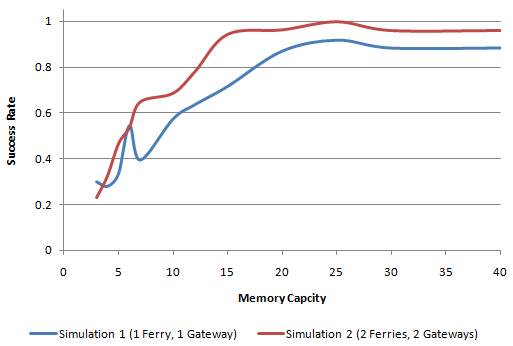
\includegraphics[width=.9\textwidth]{images/result_sccess_bothsim_128_dss}
    \caption{TODO}
    %\label{fig:moistureSensor}
\end{figure}

\subsection{Effect of Source Node Storage}

\begin{figure}[h!]
    \centering
    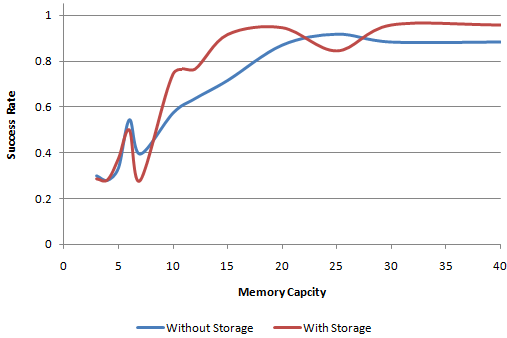
\includegraphics[width=.9\textwidth]{images/result_sccess_sim1byss_128}
    \caption{TODO}
    %\label{fig:moistureSensor}
\end{figure}


\begin{figure}[h!]
    \centering
    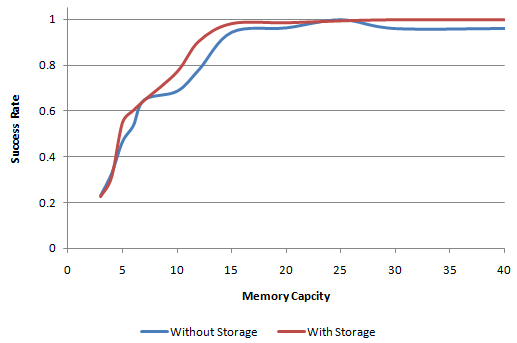
\includegraphics[width=.9\textwidth]{images/result_sccess_sim2byss_128}
    \caption{TODO}
    %\label{fig:moistureSensor}
\end{figure}

\section{Delay}

%%%%%%%%%%%%%%%%%%%%%%%%%
% References
%%%%%%%%%%%%%%%%%%%%%%%%%

%\bibliography{References}
%\addcontentsline{toc}{chapter}{\hspace{13pt}References}

%%%%%%%%%%%%%%%%%%%%%%%%%
% Appendix
%%%%%%%%%%%%%%%%%%%%%%%%%

\cleardoublepage

\begin{appendix}
\onecolumn
\section{Controller Code}

asdf

asdf
\end{appendix}

\end{document}